\chapter{Results}
\label{ch:results}

This chapter presents the results of our model training and evaluation. We tested Decision Tree, K-Nearest Neighbors (KNN), and Random Forest regressors to predict next-year home value growth using a ZIP-based test split. The following sections show how model performance varies with feature selection, test accuracy, and behavior over time.

\section{Feature selection and model comparison}

We used mutual information and f-regression to rank features, then evaluated model performance using the top-$k$ features for $k \in [1, 50]$. Figures below show the 3-fold cross-validated $R^2$ scores across feature counts.

\begin{figure}[!ht]
    \centering
    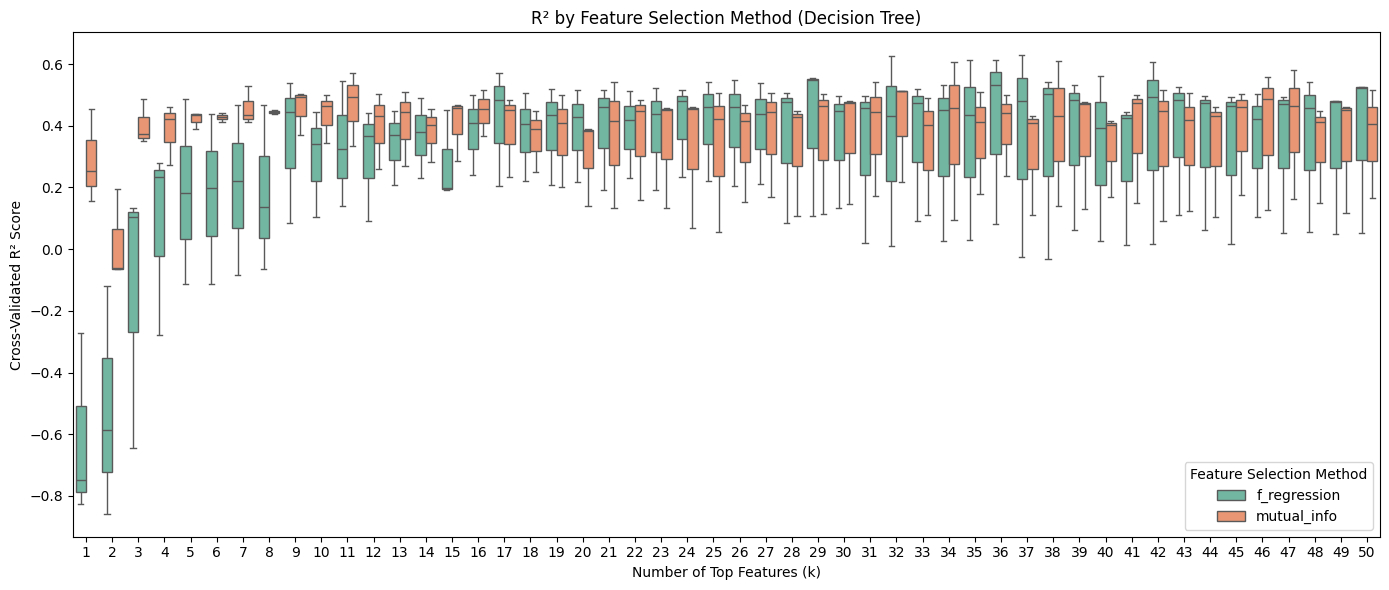
\includegraphics[width=\textwidth]{figures/box50_DT.png}
    \caption{Feature selection performance for Decision Tree}
    \caption*{\hspace{1em}}
    \label{fig:box_dt}
\end{figure}
\FloatBarrier

Decision Tree improves up to about 8–10 features, then rapidly declines. This is especially evident when using mutual information, which adds non-linear but noisy variables. The model is sensitive to irrelevant input and prone to overfitting.

\begin{figure}[!ht]
    \centering
    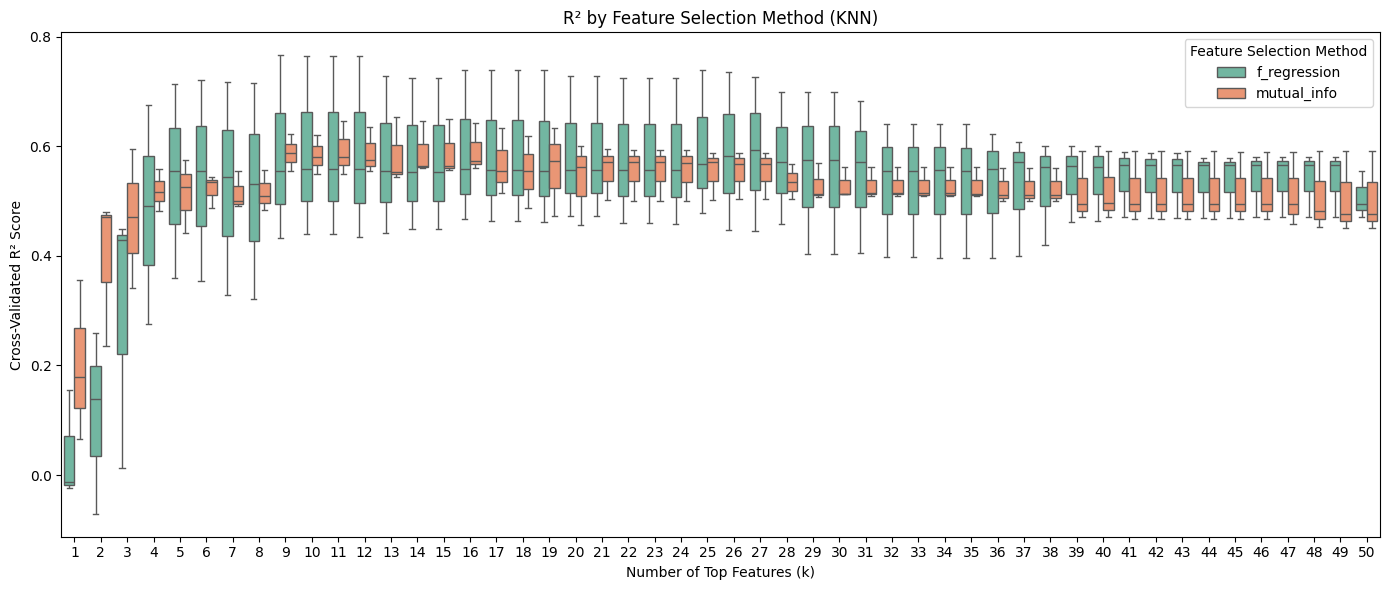
\includegraphics[width=\textwidth]{figures/box50_KNN.png}
    \caption{Feature selection performance for K-Nearest Neighbors}
    \caption*{\hspace{1em}}
    \label{fig:box_knn}
\end{figure}
\FloatBarrier

KNN performance increases up to 9 features, then plateaus. f-regression works best at low $k$, while mutual information stabilizes later. This shows that KNN benefits from smaller, more targeted feature sets and becomes unstable with excess input.

\begin{figure}[!ht]
    \centering
    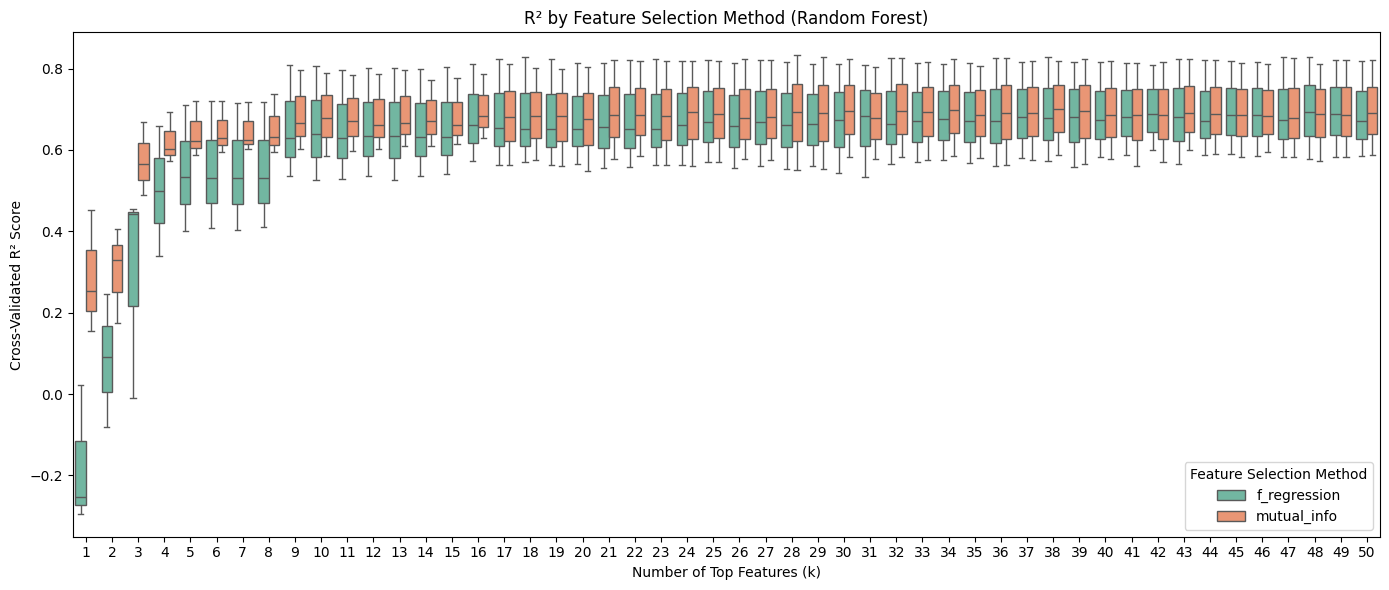
\includegraphics[width=\textwidth]{figures/box50_RF.png}
    \caption{Feature selection performance for Random Forest}
    \caption*{\hspace{1em}}
    \label{fig:box_rf}
\end{figure}
\FloatBarrier

Random Forest improves steadily up to about 16 features and holds steady beyond that. Its low variance and tolerance for redundant input reflect the model’s robustness and internal feature selection behavior.

\section{Model prediction performance}

This section evaluates how well each model predicts on unseen ZIP codes. For each model, we compare test set accuracy and generalization behavior by plotting predicted vs actual YoY values and train vs test predictions.

\subsection{Decision Tree}

\begin{figure}[!ht]
    \centering
    \subfigure[]{%
        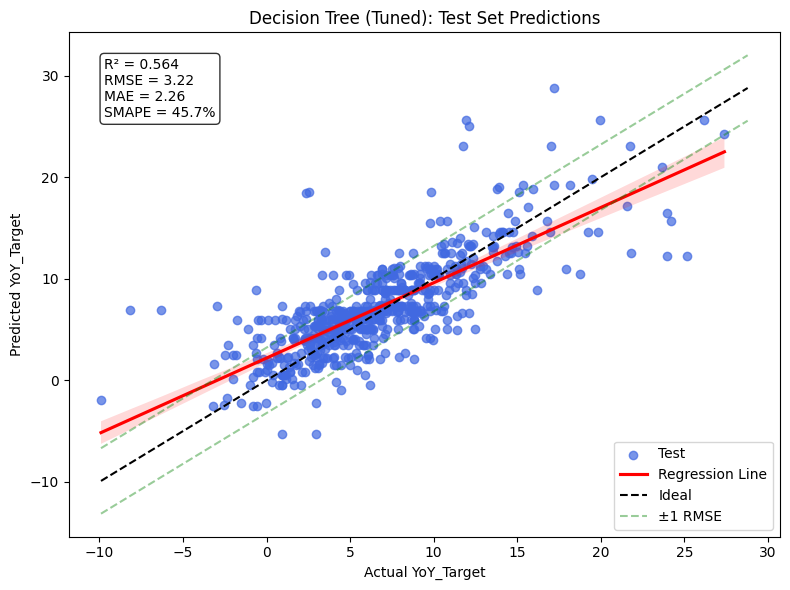
\includegraphics[width=0.48\textwidth]{figures/DT1.png}
    }\hfill
    \subfigure[]{%
        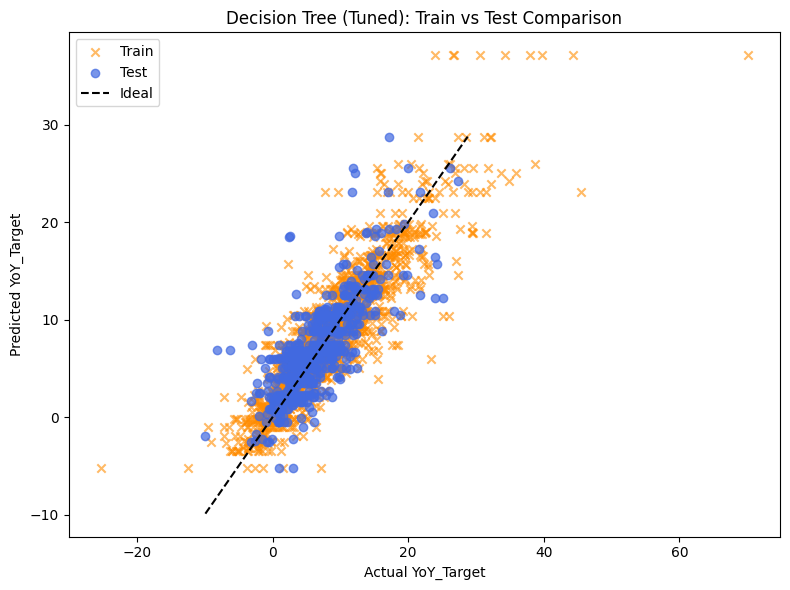
\includegraphics[width=0.48\textwidth]{figures/DT2.png}
    }
    \caption{Decision Tree test performance}
    \caption*{\hspace{1em}}
    \label{fig:dt_results}
\end{figure}
\FloatBarrier

Figure~\ref{fig:dt_results}b shows that the Decision Tree model compresses predictions toward the center of the target range. High actual values are underpredicted, and low actual values are overestimated. The regression line is noticeably flatter than the ideal diagonal, indicating a strong mean-reverting tendency. In Figure~\ref{fig:dt_results}a, the test predictions fail to reflect the wider spread in actual values, while training points follow the trend more closely. This reflects overfitting on the training set and poor generalization to unseen ZIPs, which is consistent with the model's low $R^2$ and high error rates.

\subsection{K-Nearest Neighbors (KNN)}

\begin{figure}[!ht]
    \centering
    \subfigure[]{%
        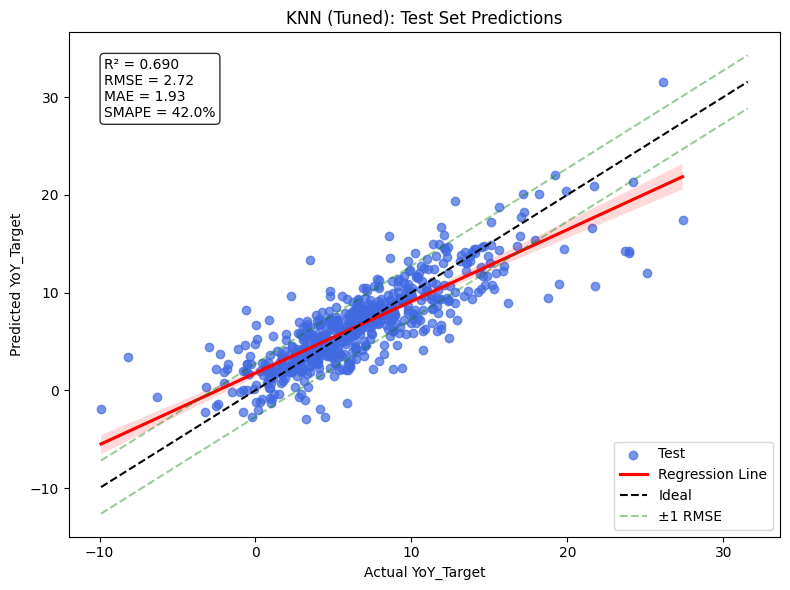
\includegraphics[width=0.48\textwidth]{figures/KNN1.png}
    }\hfill
    \subfigure[]{%
        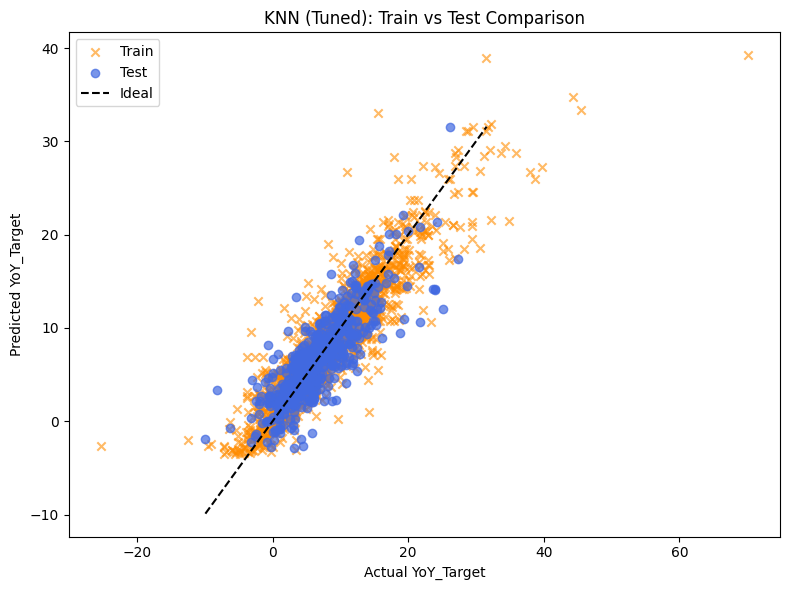
\includegraphics[width=0.48\textwidth]{figures/KNN2.png}
    }
    \caption{KNN test performance}
    \caption*{\hspace{1em}}
    \label{fig:knn_results}
\end{figure}
\FloatBarrier

KNN shows a more balanced prediction pattern. In Figure~\ref{fig:knn_results}a, most predictions fall near the regression line, though there is underprediction at the upper end and more scatter at the extremes. The central trend is captured more accurately than in Decision Tree. Figure~\ref{fig:knn_results}b shows that both train and test points follow the general diagonal trend, but test predictions are more dispersed. The model performs best when ZIPs with similar history exist in the training data, but becomes less reliable in areas with unique or high-growth patterns.

\subsection{Random Forest}

\begin{figure}[!ht]
    \centering
    \subfigure[]{%
        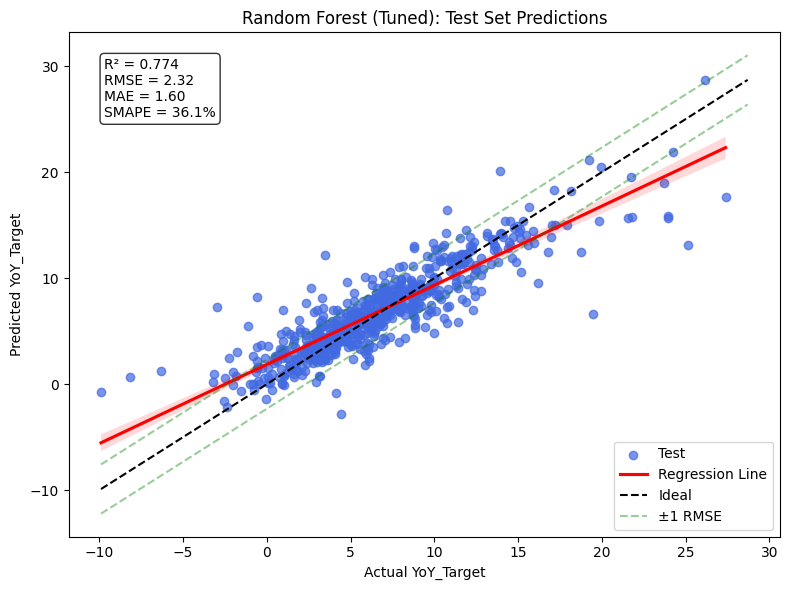
\includegraphics[width=0.48\textwidth]{figures/RF1.png}
    }\hfill
    \subfigure[]{%
        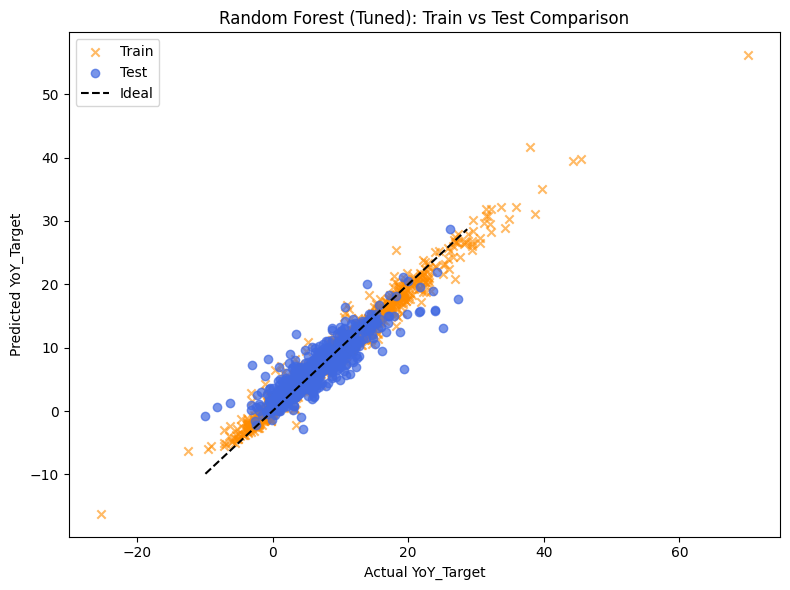
\includegraphics[width=0.48\textwidth]{figures/RF2.png}
    }
    \caption{Random Forest test performance}
    \caption*{\hspace{1em}}
    \label{fig:rf_results}
\end{figure}
\FloatBarrier

Figure~\ref{fig:rf_results}a shows that Random Forest predictions generally follow the upward trend, with the regression line reasonably close to the ideal $y = x$ line. While predictions are less dispersed than those of the other models, there is still noticeable spread, particularly at the extremes. The RMSE band captures a good portion of the points, reflecting improved but not perfect accuracy. Figure~\ref{fig:rf_results}b shows that the model performs comparably on training and test sets, with no major signs of overfitting. Overall, Random Forest offers the best balance between accuracy and generalization among the three models.

\begin{table}[!ht]
    \centering
    \caption{Test set performance summary}
    \label{tab:model_results}
    \begin{tabular}{lcccc}
        \toprule
        \textbf{Model} & \textbf{R\textsuperscript{2}} & \textbf{RMSE} & \textbf{MAE} & \textbf{SMAPE} \\
        \midrule
        Random Forest (16 features) & 0.774 & 2.32 & 1.60 & 36.2\% \\
        KNN (9 features)            & 0.690 & 2.72 & 1.93 & 42.0\% \\
        Decision Tree (8 features)  & 0.564 & 3.22 & 2.26 & 45.7\% \\
        \bottomrule
    \end{tabular}
\end{table}
\FloatBarrier

These results confirm that Random Forest was the most accurate and stable model across unseen ZIP codes, with the lowest error rates and highest $R^2$. KNN performed competitively but showed more variance on the test set. Decision Tree lagged behind due to overfitting and an inability to model the full target range.

\section{Prediction trends over time}

To evaluate how models perform across years for specific ZIP codes, we selected three ZIPs with high, median, and low ZHVI in 2024. The following figures compare actual vs predicted YoY growth over time.

\begin{figure}[!ht]
    \centering
    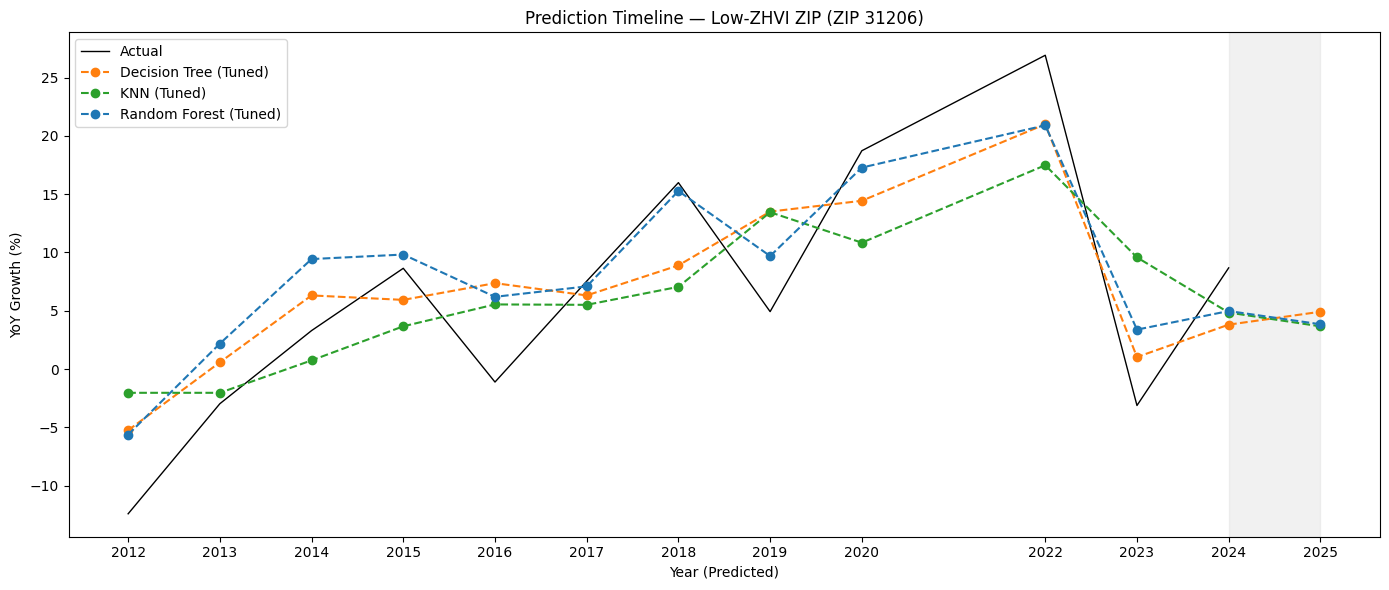
\includegraphics[width=\textwidth]{figures/timelineLow.png}
    \caption{Prediction trends over time for low-ZHVI ZIP}
    \caption*{\hspace{1em}}
    \label{fig:timeline_low}
\end{figure}
\FloatBarrier

\begin{figure}[!ht]
    \centering
    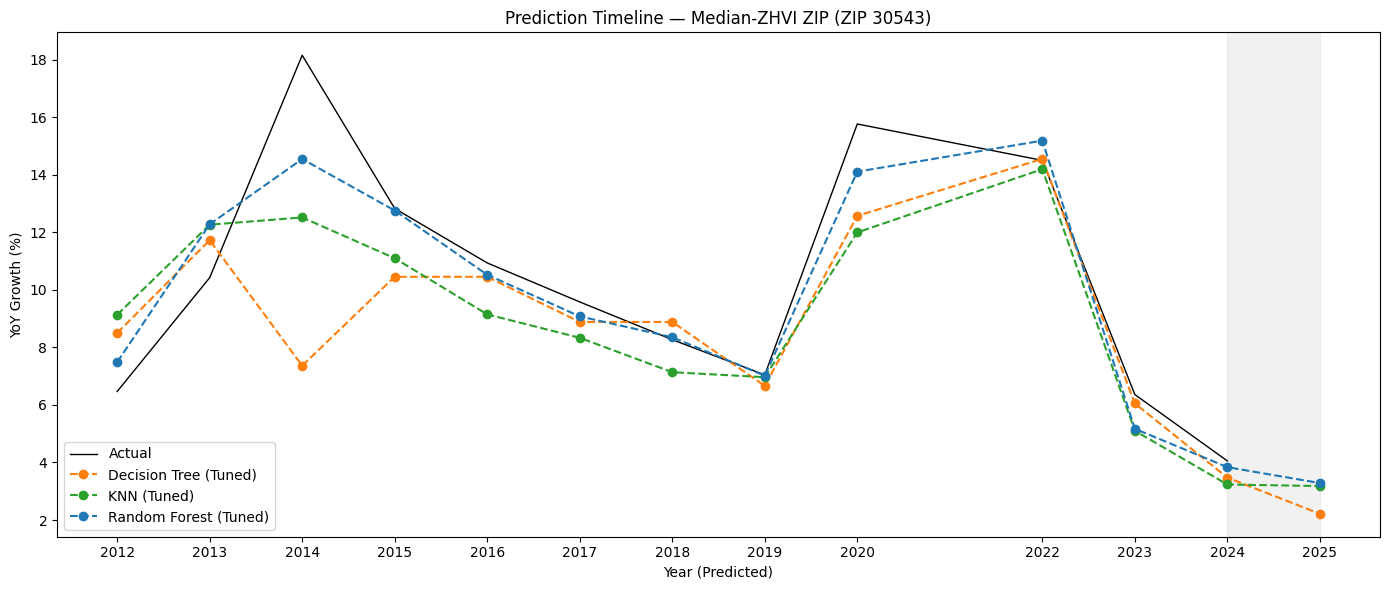
\includegraphics[width=\textwidth]{figures/timelineMedian.png}
    \caption{Prediction trends over time for median-ZHVI ZIP}
    \caption*{\hspace{1em}}
    \label{fig:timeline_median}
\end{figure}
\FloatBarrier

\begin{figure}[!ht]
    \centering
    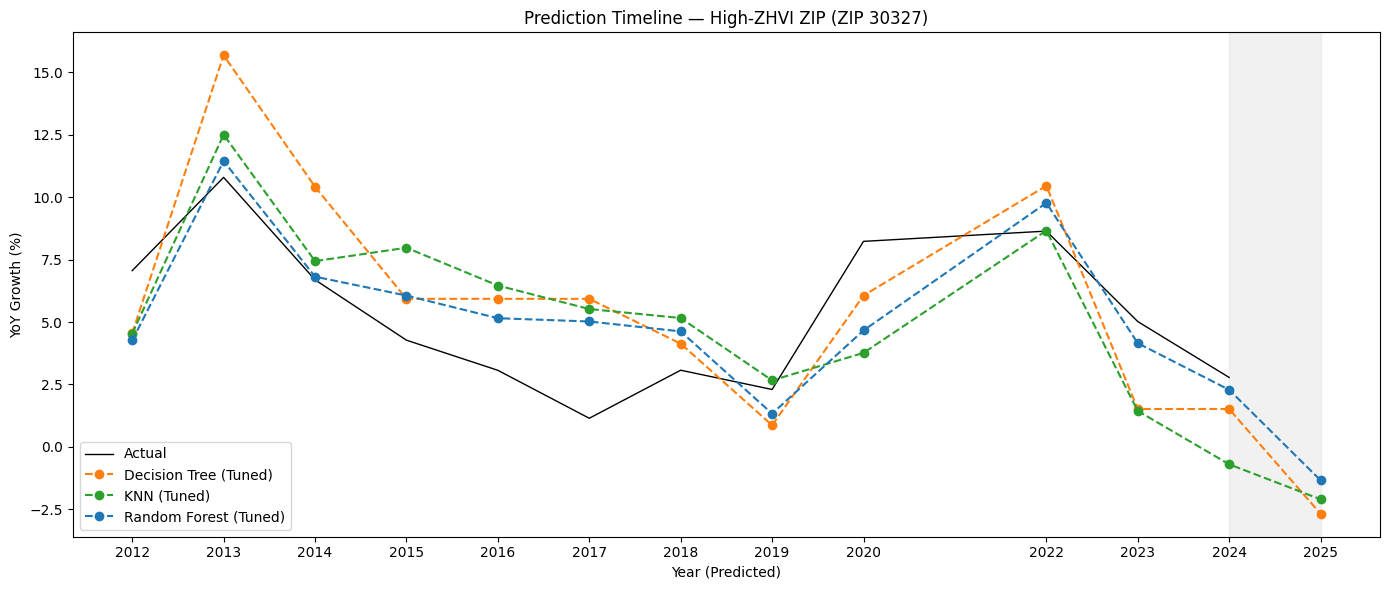
\includegraphics[width=\textwidth]{figures/timelineHigh.png}
    \caption{Prediction trends over time for high-ZHVI ZIP}
    \caption*{\hspace{1em}}
    \label{fig:timeline_high}
\end{figure}
\FloatBarrier

Across all three ZIP codes, the Random Forest model most consistently follows the actual YoY growth trend, particularly during years with noticeable dips or inflection points (e.g., 2016, 2019, 2023). In contrast, Decision Tree often smooths over or delays these changes, while KNN tends to flatten predictions and underestimates high-variance years. All models converge in the forecast period (2024–2025), but Random Forest shows closer alignment with the actual data in years prior, especially during periods of volatility.

\section{Summary}

All three models learned meaningful patterns from the data, but Random Forest consistently performed the best. It generalizes well across ZIPs, tracks yearly growth over time, and balances fit without overfitting. KNN was competitive, especially in areas with stable trends, but struggled with rapid market shifts. Decision Tree was the weakest, showing overfitting in training and poor generalization in both time and accuracy-based evaluations.
